% =====================================================================
%  CHƯƠNG 4 — TRÌNH BÀY VÀ ĐÁNH GIÁ BÀN LUẬN KẾT QUẢ
% =====================================================================
\chapter{Trình bày và đánh giá bàn luận kết quả}

Mọi so sánh trong chương dùng cùng tập test 64 mẫu (38 dương, 59,4\%), và test không tham gia vào
bất kỳ bước chọn mô hình hay chọn ngưỡng nào.

\section{Kết quả thực nghiệm}

\subsection{So sánh bốn họ mô hình}

\begin{table}[H]
\centering
\caption{Bốn họ mô hình trên test tại ngưỡng vận hành 0,788}
\label{tab:four_models}
\begin{tabular}{|l|r|r|r|r|r|l|}
\hline
\textbf{Mô hình} & \textbf{AUROC} & \textbf{AP} & \textbf{F1@0,5} & \textbf{F1@0,788} &
\textbf{MCC@0,788} & \textbf{TN/FP/FN/TP} \\
\hline
Logistic Regression  & 0,983 & 0,989 & 0,935 & 0,914 & 0,827 & 26/0/6/32 \\
Random Forest        & 0,983 & 0,991 & 0,949 & 0,960 & 0,904 & 25/1/2/36 \\
HistGradientBoosting & 0,977 & 0,987 & 0,937 & 0,907 & 0,775 & 23/3/4/34 \\
MLP                  & 0,971 & 0,982 & 0,914 & 0,895 & 0,741 & 22/4/4/34 \\
\hline
\end{tabular}
\end{table}

Random Forest là mô hình được chốt. Tại ngưỡng 0,788, nó đạt precision $= 0{,}973$,
recall $= 0{,}947$, F1 $= 0{,}960$, accuracy $= 0{,}953$, specificity $= 0{,}962$ và Brier
$= 0{,}058$. Đáng chú ý là cả bốn họ mô hình đều cho F1@0,5 khá cao (0,91--0,95) nhưng chỉ 1--2 mô
hình giữ được F1 cao khi ngưỡng dịch lên 0,788 — nghĩa là thứ hạng điểm số giữa các mô hình không
khác nhiều, khác biệt nằm ở vùng xác suất quanh ngưỡng quyết định.

\begin{figure}[H]
\centering
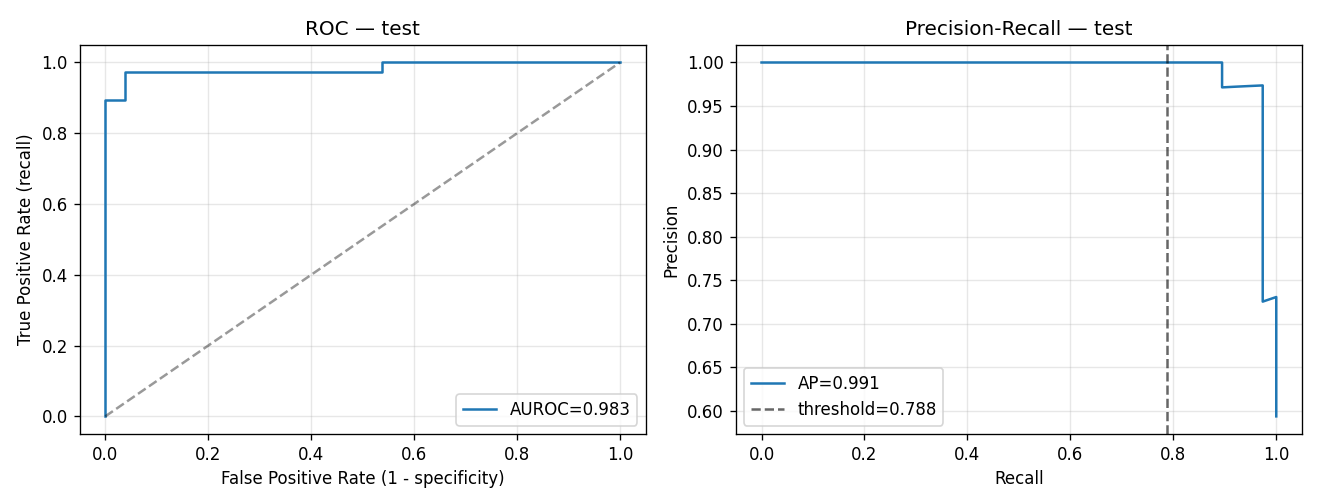
\includegraphics[width=0.72\textwidth]{figures/roc_pr_curves.png}
\caption{Đường ROC và Precision--Recall trên tập test}
\label{fig:roc_pr}
\end{figure}

\subsection{So sánh với baseline và giao thức chống thổi phồng}
\label{sec:baseline}

Đây là phần quan trọng nhất về mặt phương pháp. Nếu chỉ nhìn AUROC $\approx 0{,}98$, ta dễ kết luận
mô hình rất tốt. Nhưng đặt cạnh một baseline không dùng mô hình — lấy tỉ lệ nhãn 1 trung bình trong
train theo từng công ty (\texttt{ticker\_prior}) — mô hình gần như không hơn.

\begin{table}[H]
\centering
\caption{So sánh mô hình chốt với các hệ thống đối chứng}
\label{tab:baselines}
\begin{tabular}{|l|r|r|}
\hline
\textbf{Hệ thống} & \textbf{AUROC} & \textbf{AP} \\
\hline
model[random\_forest]                  & 0,983 & 0,991 \\
ticker\_prior (baseline không học)     & 0,986 & 0,985 \\
single\_feature[debt\_to\_assets]      & 0,889 & 0,938 \\
rule[Altman $Z'' < 1{,}1$]             & 0,758 & 0,865 \\
dummy\_most\_frequent                  & 0,500 & 0,594 \\
\hline
\end{tabular}
\end{table}

Baseline ticker-prior ngang bằng hoặc nhích hơn mô hình về AUROC (0,986 so với 0,983) và chỉ kém
hơn về AP (0,985 so với 0,991). Quy tắc Altman $Z''$ đạt AUROC 0,758 — thấp hơn rõ rệt nhưng dùng
công thức công khai, không học tham số và không cần huấn luyện. Để tách phần "nhớ mặt công ty" khỏi
năng lực tổng quát hoá, khóa luận đánh giá lại theo \texttt{GroupKFold} (giữ trọn một công ty ra
ngoài train trong mỗi fold).

\begin{table}[H]
\centering
\caption{In-domain so với cross-company (GroupKFold)}
\label{tab:cross_company}
\begin{tabular}{|l|r|r|r|r|}
\hline
\textbf{Mô hình} & \textbf{AUROC in-domain} & \textbf{AP in-domain} &
\textbf{AUROC cross-co.} & \textbf{AP cross-co.} \\
\hline
Random Forest        & 0,983 & 0,991 & 0,933 & 0,957 \\
Logistic Regression  & 0,983 & 0,989 & 0,912 & 0,942 \\
HistGradientBoosting & 0,977 & 0,987 & 0,926 & 0,953 \\
MLP                  & 0,971 & 0,982 & 0,789 & 0,832 \\
\hline
\end{tabular}
\end{table}

Hai điểm cần nói thẳng. Thứ nhất, khi giữ công ty ra ngoài, AUROC của mô hình chốt giảm từ 0,983
xuống 0,933 — mức sụt này cho biết một phần đáng kể hiệu năng in-domain đến từ việc nhận diện công
ty. Thứ hai, MLP sụt mạnh nhất (0,971 $\rightarrow$ 0,789): mạng nơ-ron tận dụng tốt các đặc trưng
gần như bất biến theo công ty nên khi công ty bị giữ trọn ra ngoài thì mất chỗ dựa. Thêm một phép
thử khắt khe là \texttt{Leave-One-Company-Out}: AUROC trung bình chỉ 0,628.

\subsection{Ngưỡng quyết định theo chi phí kỳ vọng}

\begin{table}[H]
\centering
\caption{Ngưỡng theo F1 và theo chi phí kỳ vọng}
\label{tab:threshold}
\begin{tabular}{|l|r|r|r|r|r|}
\hline
\textbf{Tập} & \textbf{Ngưỡng best-F1} & \textbf{F1} & \textbf{Precision} & \textbf{Recall} &
\textbf{Chi phí kỳ vọng} \\
\hline
validation & 0,788 & 0,976 & 1,000 & 0,952 & 5,0 \\
test       & 0,783 & 0,974 & 0,974 & 0,974 & 6,0 \\
\hline
\end{tabular}
\end{table}

Điểm cần nói thẳng: ngưỡng triển khai 0,788 lấy từ validation, trong khi trên test ngưỡng tối ưu chi
phí là 0,783. Chỉ lệch 0,005 nhưng trên 64 mẫu nó biến 1 dương tính thật thành bỏ sót: tại 0,788,
ma trận nhầm lẫn là TN/FP/FN/TP $= 25/1/2/36$; tại 0,783 là $25/1/1/37$. Đây là biểu hiện rõ của việc
chọn ngưỡng trên một tập nhỏ rồi áp lên tập khác — không sai về giao thức, nhưng cần đọc kèm khoảng
tin cậy thay vì tin vào một con số duy nhất.

\subsection{Kiểm định ý nghĩa thống kê và độ nhạy theo định nghĩa nhãn}

Để tránh kết luận "mô hình tốt hơn" chỉ dựa vào chênh lệch điểm số, khóa luận kiểm định trên cùng 64
mẫu test: DeLong \cite{delong1988} cho $\Delta$AUROC và paired bootstrap (2.000 vòng) cho
$\Delta$AP.

\begin{table}[H]
\centering
\caption{Kiểm định mô hình chốt so với các hệ thống khác}
\label{tab:significance}
\begin{tabular}{|l|r|r|r|l|r|}
\hline
\textbf{So sánh (A $-$ B)} & \textbf{$\Delta$AUROC} & \textbf{p (DeLong)} & \textbf{$\Delta$AP} &
\textbf{CI95 $\Delta$AP} & \textbf{p (bootstrap)} \\
\hline
RF $-$ ticker\_prior        & $-0{,}0030$ & 0,755  & $+0{,}0061$ & $[-0{,}005; +0{,}022]$ & 0,344 \\
RF $-$ single\_feature      & $+0{,}0941$ & 0,0076 & $+0{,}0528$ & $[+0{,}018; +0{,}097]$  & 0,001 \\
RF $-$ dummy\_most\_frequent& $+0{,}4828$ & $<0{,}001$ & $+0{,}3970$ & $[+0{,}379; +0{,}406]$ & $<0{,}001$ \\
\hline
\end{tabular}
\end{table}

Kết quả then chốt: mô hình chốt không khác baseline ticker-prior về ý nghĩa thống kê (p $=$ 0,755 cho
AUROC; p $=$ 0,344 cho AP, khoảng tin cậy chứa 0). Cần đọc đúng: "không khác biệt" nghĩa là dữ liệu
chưa đủ để khẳng định mô hình hơn, không phải bằng chứng mô hình kém. Với $n = 64$, khoảng tin cậy
vốn rộng.

\subsection{Kiểm chứng độ nhạy theo định nghĩa nhãn}
\label{sec:nhan}

Nhóm dựng lại toàn bộ split bằng ba định nghĩa nhãn công khai, tái lập được (\texttt{stress\_signals},
Altman $Z''$, forward 4 quý) và chạy lại đúng một mô hình.

\begin{table}[H]
\centering
\caption{Kiểm chứng độ nhạy theo định nghĩa nhãn}
\label{tab:label_sensitivity}
\begin{tabular}{|l|r|r|r|r|r|}
\hline
\textbf{Định nghĩa nhãn} & \textbf{Dương (test)} & \textbf{Khớp nhãn gốc} &
\textbf{AUROC mô hình} & \textbf{AUROC ticker-prior} & \textbf{Cross-co. AP} \\
\hline
original (nhãn gốc) & 59,4\% & 100\% & 0,983 & 0,986 & 0,958 \\
stress\_signals     & 42,2\% & 74,4\%& 0,909 & 0,960 & 0,610 \\
altman\_z           & 31,2\% & 63,9\%& 0,999 & 0,991 & 0,460 \\
forward\_4q         & 48,4\% & 66,7\%& 0,836 & 0,911 & 0,582 \\
\hline
\end{tabular}
\end{table}

Luận điểm "mô hình không vượt baseline nhớ mặt công ty" xuất hiện ở 3/3 định nghĩa nhãn tái lập được
— đây là bằng chứng mạnh nhất của khóa luận: kết luận không phụ thuộc vào cách gán nhãn. Đồng thời,
cross-company AP sụt rất mạnh ở các định nghĩa khác (0,46--0,61), xác nhận lại rằng phần lớn hiệu
năng in-domain đến từ thực thể chứ không từ động lực suy giảm của từng quý.

\subsection{Thực nghiệm phản biện}

Để trả lời câu hỏi "có phải do chọn họ mô hình nên chưa hơn baseline?", khóa luận chạy thêm hai đối
chứng ngoài pipeline chính: một SVM tuyến tính nhẹ (LiteSVM, cài bằng numpy) và XGBoost
\cite{chen2016}.

\begin{table}[H]
\centering
\caption{Mô hình chốt so với LiteSVM và XGBoost}
\label{tab:defense}
\begin{tabular}{|l|r|r|l|}
\hline
\textbf{Mô hình} & \textbf{Test AUROC} & \textbf{Test AP} & \textbf{TN/FP/FN/TP} \\
\hline
LiteSVM (SGD hinge + class\_weight) & 0,965 & 0,976 & 26/0/19/19 \\
XGBoost (scale\_pos\_weight + early stop) & 0,982 & 0,990 & 26/0/4/34 \\
Random Forest (khóa luận) & 0,983 & 0,991 & 25/1/2/36 \\
\hline
\end{tabular}
\end{table}

XGBoost đạt AUROC/AP tương đương Random Forest trong khi không có FP nào (bỏ sót 4) — việc thay
boosting bằng bagging không tạo khác biệt lớn trên bộ dữ liệu này. Khóa luận cũng chạy thí nghiệm xử
lý mất cân bằng trên dữ liệu thật (SMOTE \cite{chawla2002}, SMOTE+ENN, RandomUnderSampler,
class\_weight) đặt trong \texttt{imblearn.pipeline.Pipeline} \cite{lemaitre2017} để không chạm test;
kỹ thuật tốt nhất (\texttt{smote\_enn}, AP 0,9683 so với 0,9588 của đối chứng) nhưng $\Delta$AP
$= +0{,}0095$ với p $= 0{,}21$ — chưa đủ căn cứ. Một chi tiết đáng lưu ý: vì lớp 1 chiếm đa số
(62\%), SMOTE ở đây sinh thêm mẫu lớp 0, tức can thiệp ngược với thực hành phổ biến — thêm một lý do
để mất cân bằng không phải nút thắt của bài toán này.

\section{Phân tích độ quan trọng đặc trưng và SHAP}

\subsection{Permutation importance}

Khóa luận dùng permutation importance \cite{fisher2019} (hoán vị từng cột, đo mức giảm AUROC). Kết
quả trên validation ở Bảng~\ref{tab:importance}.

\begin{table}[H]
\centering
\caption{Độ quan trọng đặc trưng (permutation, $\Delta$AUROC trên validation)}
\label{tab:importance}
\begin{tabular}{|r|l|r|}
\hline
\textbf{Hạng} & \textbf{Đặc trưng} & \textbf{$\Delta$AUROC (val)} \\
\hline
1 & gross\_margin\_latest            & 0,008 \\
2 & receivables\_to\_sales\_latest   & 0,001 \\
3 & working\_capital\_to\_assets     & 0,001 \\
4 & operating\_margin\_latest        & 0,001 \\
5 & net\_margin\_latest              & 0,000 \\
6 & retained\_to\_assets\_latest     & 0,000 \\
\hline
\end{tabular}
\end{table}

Các $\Delta$AUROC đều rất nhỏ ($\leq 0{,}008$) — nghĩa là khi công ty đã được nhận diện, không đặc
trưng đơn lẻ nào còn đóng góp lớn. Đặc trưng dẫn đầu là \texttt{gross\_margin\_latest} (biên lợi
nhuận gộp), hợp lý với ngành bán lẻ vì đây là tỷ số phản ứng nhanh nhất với áp lực giá và cơ cấu
hàng tồn.

\begin{figure}[H]
\centering
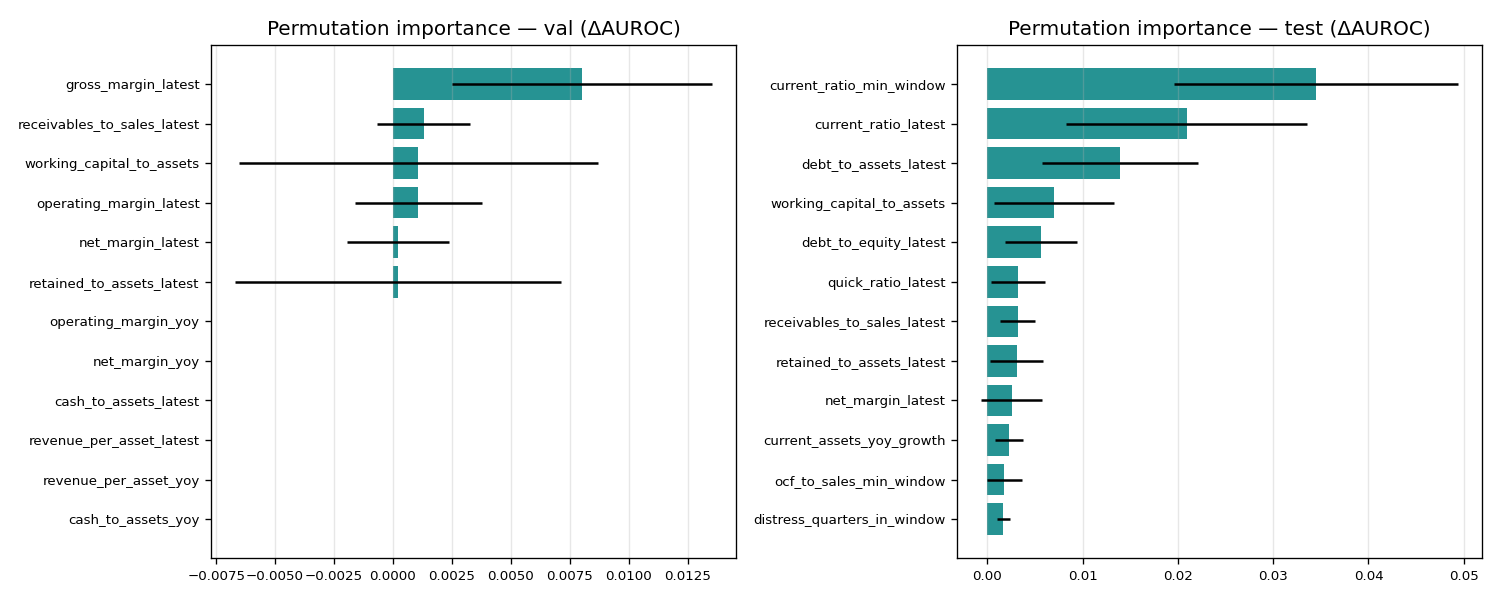
\includegraphics[width=0.74\textwidth]{figures/feature_importance.png}
\caption{Độ quan trọng đặc trưng (permutation importance)}
\label{fig:importance}
\end{figure}

\subsection{Ablation theo nhóm đặc trưng}

\begin{table}[H]
\centering
\caption{Ablation theo nhóm đặc trưng (test)}
\label{tab:ablation}
\begin{tabular}{|l|r|r|r|r|}
\hline
\textbf{Biến thể} & \textbf{Số đặc trưng} & \textbf{AUROC} & \textbf{AP} & \textbf{F1} \\
\hline
Tất cả đặc trưng        & 47 & 0,983 & 0,991 & 0,949 \\
Bỏ nhóm ratios\_latest  & 33 & 0,966 & 0,982 & 0,949 \\
Bỏ nhóm ratios\_yoy     & 33 & 0,974 & 0,985 & 0,949 \\
Bỏ nhóm growth          & 37 & 0,985 & 0,993 & 0,949 \\
Bỏ nhóm path            & 41 & 0,977 & 0,987 & 0,949 \\
Chỉ mẫu $\geq 5$ quý     & 47 & 0,987 & 0,993 & 0,949 \\
\hline
\end{tabular}
\end{table}

Ablation cho thấy F1 test gần như không đổi (0,949) ở mọi biến thể, còn AUROC dao động trong khoảng
$\pm 0{,}02$ — kết luận không nhạy với việc bỏ nguyên một nhóm đặc trưng. Bỏ nhóm
\texttt{ratios\_latest} làm AUROC giảm nhiều nhất (0,983 $\rightarrow$ 0,966), cho thấy giá trị tỷ số
tại quý gần nhất là phần thông tin cốt lõi. Một cảnh báo kỹ thuật đi kèm: đa cộng tuyến cao —
33/47 đặc trưng có VIF $>$ 10, nặng nhất là \texttt{debt\_to\_equity} và các cột \texttt{cash\_*}.
Với mô hình tuyến tính, VIF cao làm hệ số bất ổn và khó diễn giải; với mô hình cây thì ít ảnh hưởng
đến dự báo nhưng vẫn làm độ quan trọng bị chia đều giữa các cột tương quan.

\subsection{Giải thích cục bộ bằng SHAP}

Ngoài độ quan trọng toàn cục, khóa luận dùng KernelSHAP tự cài đặt \cite{lundberg2017} để giải thích
từng ca dự báo: với mỗi mẫu, tính đóng góp của từng đặc trưng vào độ lệch so với giá trị nền. Phần
này được dùng chủ yếu cho ứng dụng minh hoạ và kiểm tra tính hợp lý, không dùng để chọn mô hình —
lý do là SHAP tính trên mô hình đã fit, nếu dùng để chọn cây sẽ quay lại đúng vấn đề thổi phồng
in-domain đã nêu ở mục~\ref{sec:baseline}.

\begin{figure}[H]
\centering
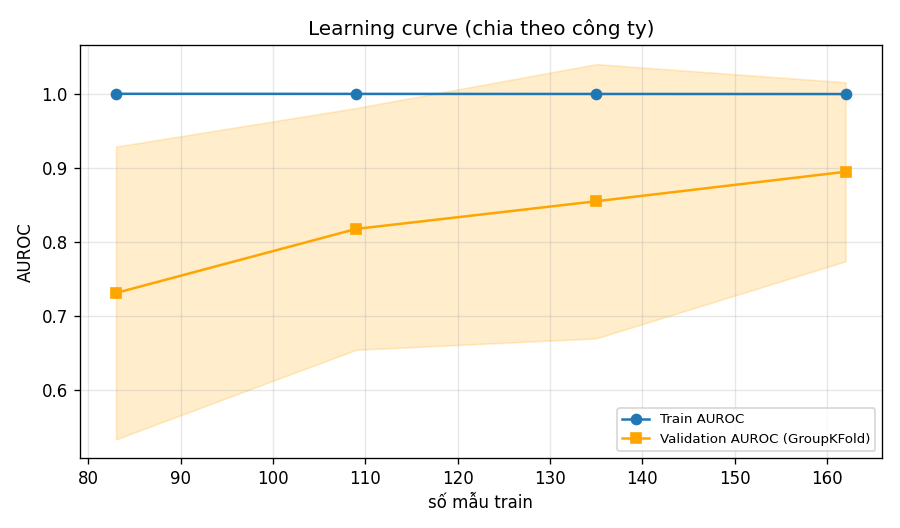
\includegraphics[width=0.76\textwidth]{figures/learning_curve.png}
\caption{Learning curve khi chia theo công ty}
\label{fig:learning_curve}
\end{figure}

\section{Phân tích lỗi và thảo luận}

\subsection{Phân tích lỗi (error analysis)}

Trên test, mô hình chốt sai 3/64 mẫu. Bảng~\ref{tab:errors} truy vết từng ca tới chỉ tiêu cụ thể.

\begin{table}[H]
\centering
\caption{Ba mẫu dự đoán sai trên tập test}
\label{tab:errors}
\begin{tabular}{|l|l|r|l|r|r|r|r|}
\hline
\textbf{Mẫu} & \textbf{Cty} & \textbf{Thực} & \textbf{Dự đoán} & \textbf{P} &
\textbf{current\_r.} & \textbf{WC/TA} & \textbf{net\_m.} \\
\hline
HD-2024Q2   & HD   & 1 & 0 (FN) & 0,783 & 1,34 & 0,10 & 0,099 \\
DG-2025Q2   & DG   & 0 & 1 (FP) & 0,798 & 1,23 & 0,05 & 0,038 \\
FIVE-2024Q3 & FIVE & 1 & 0 (FN) & 0,174 & 1,63 & 0,11 & 0,040 \\
\hline
\end{tabular}
\end{table}

Ba ca này lộ ra đúng bản chất vấn đề. HD-2024Q2 là bỏ sót sát ngưỡng: HD có 100\% quý mang nhãn 1,
nhưng quý này các tỷ số lại khá hơn (net\_margin 0,099; debt/assets 0,98) nên xác suất 0,783 nằm
ngay dưới ngưỡng 0,788 — mô hình gần như dựa vào danh tính công ty chứ không vào tín hiệu của quý.
FIVE-2024Q3 là bỏ sót nặng (0,174): đây là lỗi đáng lo nhất, vì mô hình không hề thấy dấu hiệu nào.
DG-2025Q2 là báo động giả (0,798) ở một công ty có nhãn lẫn lộn. Điểm chung: cả ba mẫu đều thuộc các
công ty có tỉ lệ nhãn trung gian, nơi ranh giới quyết định mờ.

\begin{figure}[H]
\centering
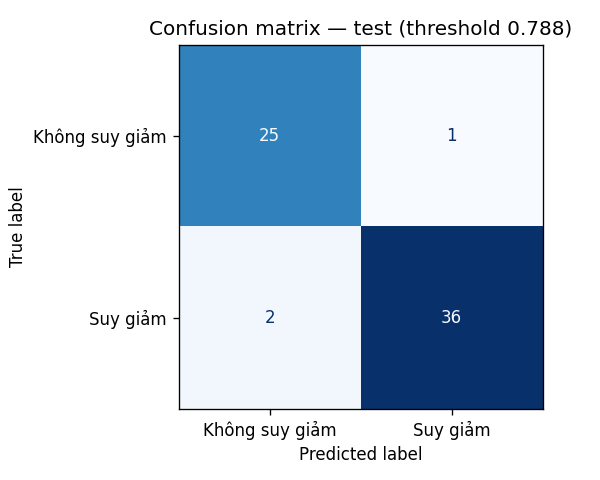
\includegraphics[width=0.52\textwidth]{figures/confusion_matrix.png}
\caption{Ma trận nhầm lẫn của mô hình chốt trên tập test}
\label{fig:confusion}
\end{figure}

\subsection{Rào cản kỹ thuật khi triển khai thực tế}

\begin{enumerate}
\item \textbf{Độ trễ dữ liệu theo quý.} Đầu vào là báo cáo quý đã công bố. 10-Q thường được nộp
      sau khi quý kết thúc khoảng 40 ngày, 10-K có kiểm toán; mọi đặc trưng dùng mốc
      \texttt{available\_on} $=$ ngày \texttt{filed}. Điều đó có nghĩa dự báo chỉ có thể đưa ra SAU
      khi báo cáo được nộp, mô hình không thể cảnh báo sớm hơn chính dữ liệu. Tệ hơn, các tỷ số kế
      toán là chỉ báo trễ: khi chúng xấu đi thì vấn đề thường đã xảy ra rồi.
\item \textbf{Rò rỉ thông tin cấp thực thể.} Đây là rủi ro lớn nhất về phương pháp. Nếu chia tập
      ngẫu nhiên theo mẫu, cùng một công ty xuất hiện ở cả train lẫn test và mô hình chỉ cần nhớ
      mặt công ty là đủ đạt điểm cao giả tạo. Khóa luận tránh bằng chia theo thời gian, GroupKFold,
      LOCO và luôn so với baseline ticker-prior.
\item \textbf{Chi phí sai không đối xứng.} Trong ứng dụng đầu tư/cho vay, một false negative (bỏ
      sót doanh nghiệp sắp suy giảm) đắt hơn một false positive. Khóa luận xử lý bằng ngưỡng tối ưu
      chi phí, nhưng giả định $C_{FN} = 5$ là con số minh hoạ, không phải con số đo từ thị trường.
\item \textbf{Nhãn mục tiêu không tái tạo được.} Không quy tắc kế toán đơn giản nào khớp nhãn gốc
      quá 74,7\%. Điều này giới hạn khả năng kiểm chứng độc lập và buộc khóa luận phải kiểm chứng
      độ nhạy bằng các định nghĩa nhãn thay thế.
\item \textbf{Nguy cơ overfitting.} Random Forest đạt AUROC train 1,000 nhưng validation 0,965
      (gap 0,034); learning curve chia theo công ty cho gap khoảng 0,105 AUROC. Với 212 mẫu train và
      47 đặc trưng, đây là mức overfit cần theo dõi, và là lý do khóa luận không dùng cấu hình tinh
      chỉnh phức tạp.
\end{enumerate}

\subsection{Ý nghĩa thực tiễn và hạn chế}

Giá trị thực dụng rõ nhất không nằm ở con số AUROC 0,983, mà ở hai thứ khác. Thứ nhất là khả năng tự
động hoá bóc tách: thay vì đọc 8 $\times$ 44 báo cáo, pipeline lấy thẳng \texttt{companyfacts},
chuẩn hoá kỳ kế toán, tính 47 đặc trưng và gán nhãn, tất cả tái lập được từ một lệnh. Thứ hai là
phát hiện trung thực về rò rỉ cấp thực thể: bất kỳ ai triển khai dự báo suy giảm trên bộ dữ liệu ít
thực thể đều cần biết rằng AUROC in-domain có thể cao phần lớn do nhận diện công ty.

Về hạn chế: cỡ mẫu nhỏ và chỉ 8 thực thể nên mọi kết luận phải đi kèm khoảng tin cậy và không suy
rộng ra toàn ngành; chuỗi thời gian bị chồng lấn giữa các mẫu liên tiếp nên số quan sát độc lập thực
tế nhỏ hơn 324; nhãn gốc không tái tạo được; đơn vị tiền chỉ là quy đổi minh hoạ; và bộ dữ liệu
không chứa sự kiện phá sản thật, nên kết quả không thể diễn giải thành năng lực dự báo phá sản.



